\chapter{Fundamentals of the Computational Methods} % Main chapter title

\label{Chapter3} % Change X to a consecutive number; for referencing this chapter elsewhere, use \ref{ChapterX}


\section{SAFT-$\gamma$ Mie Force Field}

\subsection{SAFT-VR Mie EoS}

The SAFT-VR Mie equation of state \cite{lafitte2013} is the basis for the SAFT-$\gamma$ Mie coarse grained force field \cite{avendano2011}. This EoS was initially developed to describe chain molecule formed from fused Mie segments using the Mie attractive and repulsive potential. The Mie potential is a type of generalized Lennard-Jones potential that can be used to describe explicitly repulsive interactions of different hardness/softness and attractive interactions of different ranges, and is given by:
\begin{equation}
U_{Mie}(r) = \epsilon\frac{\lambda_r}{\lambda_r - \lambda_a} \left(\frac{\lambda_r}{\lambda_a} \right)^{\left( \frac{\lambda_a}{\lambda_r - \lambda_a} \right)}
\left[ \left(\frac{\sigma}{r} \right)^{\lambda_r} - \left(\frac{\sigma}{r} \right)^{\lambda_a} \right]
\label{eqn:miepotential}
\end{equation}
where $\epsilon$ is the potential well depth, $\sigma$ is the segment diameter, r is the distance between the spherical segments, $\lambda_r$ is the repulsive exponent and $\lambda_a$ is the attractive exponent. This equation uses the \citeonline{bh1976} high perturbation expansion of the Helmholtz free energy up to third order and an improved expression for the  radial distribution function (RDF) of Mie monomers at contact to obtain a equation able to give an accurate theoretical description of the vapor-liquid equilibrium and second derivative properties \cite{lafitte2013}. For a non-associating fluid, the Helmholtz free energy is:
\begin{equation}
\frac{A}{N\kappa_{b}T} = a = a^{IDEAL} + a^{MONO} + a^{CHAIN}
\label{eqn:miehelm}
\end{equation}

\subsubsection{Ideal Contribution}

The ideal contribution for a mixture is given by:
\begin{equation}
a^{IDEAL} = \sum_{i=1}^{N_{c}} x_{i}\ln{(\rho_{i}{\Lambda_{i}}^3)} -1
\label{eqn:aideal}
\end{equation}
where $x_{i}=N_{i}/N$ is the molar fraction of component i, $\rho_{i}=N_{i}/V$ is the number density, $N_{i}$ is the number of molecules of each component and $\Lambda_{i}^3$ is de Broglie wavelength. 

\subsubsection{Monomer Contribution}

The monomer contribution describes the interactions between Mie segments and can be expressed for a mixture as:
\begin{equation}
a^{MONO} = \left(\sum_{i=1}^{N_{c}} x_{i}m_{s,i} \right)a^{M}
\label{eqn:amonomer}
\end{equation}

In the equation above, $m_{s,i}$ is the number of spherical segments making up the molecule i and $a^{M}$  is the monomer dimensionless Helmholtz free energy and it is expressed as a third order perturbation expansion in the inverse temperature \cite{bh1976}:
\begin{equation}
a^{M} = a^{HS}+\beta{a_{1}}+\beta{a_{2}}^2+\beta{a_{3}}^3 
\label{eqn:aM}
\end{equation}
where $\beta=\kappa_{b}T$ and $a^{HS}$ is the hard-sphere dimensionless Helmholtz free energy for a mixture :
\begin{equation}
a^{HS} = \frac{6}{\pi\rho_{s}}\left[\left(\frac{\zeta^3_2}{\zeta^2_3}-\zeta_0 \right)\ln(1-\zeta_3)+\frac{3\zeta_{1}\zeta_{2}}{1-\zeta_3}+ \frac{\zeta^3_2}{\zeta_{3}(1-\zeta_3)^2}\right]
\label{eqn:hs}
\end{equation}

The variable $\rho_{s}=\rho\sum_{i}^{N_c} x_{i}m{s,i}$ is the total number density of spherical segments and $\zeta_l$ are the moments of the number density:
\begin{equation}
\zeta_l = \frac{\pi\rho_s}{6}\left(\sum_{i=1}^{N_c} x_{s,i}d^l_{ii} \right), l = 0,1,2,3
\label{eqn:zetal}
\end{equation}
where $x_{s,i}$ is the mole fraction of the segments and is related through the mole fraction of component i ($x_i$) by:
\begin{equation}
x_{s,i} = \frac{m_{s,i}x_i}{\sum_{k=1}^{N_c} m_{s,k}x_{k} }
\label{eqn:xsi}
\end{equation}


The effective hard-sphere diameter $d_{ii}$ for the segments is:
\begin{equation}
d_{ii} =\int_{0}^{\sigma_{ii}} ( 1 - \exp(-\beta U^{Mie}_{ii}(r)) ) dr
\label{eqn:diameter}
\end{equation}


The integral in Eq. \eqref{eqn:diameter} is normally obtained by means of Gauss-Legendre with a 5-point quadrature \cite{papa2014}. The detailing of terms of Eq. \eqref{eqn:amonomer} can be found in \citeonline{lafitte2013}.

\subsubsection{Chain Contribution}
The chain formation of $m_{s}$ tangentially bonded Mie segments contribution is based on the first-order pertubation theory (TPT1)  \cite{papa2014} and can be expressed as:
\begin{equation}
a^{CHAIN} =-\sum_{i=1}^{N_{c}} x_{i}(m_{s,i} - 1)\ln(g_{ii}^{Mie}(\sigma_{ii}))
\label{eqn:achain}
\end{equation}


The $g_{ij}^{Mie}(\sigma_{ij})$ term correspond to the value of the radial distribution function (RDF) of the hypothetical Mie system evaluated at the effective diameter and can be obtained with the perturbation expansion:
\begin{equation}
\begin{aligned}
g_{ij}^{Mie}(\sigma_{ij}) =g_{d,ij}^{HS}(\sigma_{ij})\exp[\beta\epsilon g_{1,ij}(\sigma_{ij})/g_{d,ij}^{HS}(\sigma_{ij}) + (\beta\epsilon)^{2} g_{2,ij}(\sigma_{ij})/g_{d,ij}^{HS}(\sigma_{ij})]
\end{aligned}
\label{eqn:gmie}
\end{equation}


The other terms in the equations above are explicitly exposed in the original article \cite{lafitte2013}. 

\subsubsection{Ring Contribution}
There are two forms for the Helmholtz free energy for rings formed from $m_{s}$ tangentially bonded segments in the literature. The first one  \cite{lafitte2012} considered that the difference between a chain and a ring molecule is that the latter has one more bond that is connecting the first segment to the last. With this assumption, the Eq. \eqref{eqn:achain} can be adapted to rings by:
\begin{equation}
a^{RING} =-\sum_{i=1}^{N_{c}} x_{i}m_{s,i}\ln(g_{ii}^{Mie}(\sigma_{ii}))
\label{eqn:aringlafitte}
\end{equation}

According to \citeonline{lafitte2012}, Eq. \eqref{eqn:aringlafitte} needs an additional parametrization with molecular simulation data so the EoS can  be used in molecular simulations, but this procedure is not the necessary for chain molecules. Recently \citeonline{muller2017} tried to correct this inconsistency by means of developing the ring free energy based on the work of \citeonline{muller1993} who obtained rigorous expressions for hard fluids with molecular geometries of rings of $m_s=3$. The final expression developed for the ring dimensionless Helmholtz free energy is:
\begin{equation}
a^{RING} =-\sum_{i=1}^{N_{c}} x_{i}(m_{s,i}-1+\chi_{i}\eta_{i})\ln(g_{ii}^{Mie}(\sigma_{ii}))
\label{eqn:aringmuller}
\end{equation}
$\eta_{i}=m_{s,i}\rho_{i}\sigma_{ii}^{3}/6$ is the packing fraction and $\chi_{i}$ is a parameter which depends on $m_{s,i}$ and on the geometry of the ring of each component i. For a value of $\chi=0$ Eq. \eqref{eqn:aringmuller} is equal to Eq. \eqref{eqn:achain}. Meanwhile, the equation corresponds to a hard sphere system of triangles when $\chi=1.3827$. \citeonline{muller2017} also calculated values of $\zeta$ for $m_{s}=3,m_{s}=4,m_{s}=5,m_{s}=7$ with pseudo-experimental data from molecular dynamics (MD) for a defined pure fluid. The values of $\chi$ for each geometry estimated can be seen in the \figref{ringqsi}.
\begin{figure}[th]
\centering
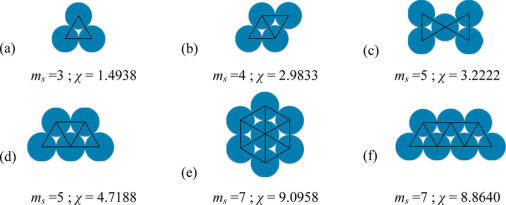
\includegraphics[scale=0.8]{Figures/mullergeo.jpg}
\caption{Values for parameter $\chi$ according to the ring geometry \cite{muller2017}}
\label{ringqsi}
\end{figure}

\subsubsection{Combining rules for the intermolecular potential parameters}
\citeonline{lafitte2013} also suggested mixing rules for the potential parameters based on Lorentz-Berthelot combining rules \cite{rowlinson}:
\begin{equation}
\sigma_{ij} =\frac{\sigma{ii}+\sigma{jj}}{2}
\label{eqn:sigmamix}
\end{equation}
\begin{equation}
\lambda_{k,ij} -3 =\sqrt{(\lambda_{k,ii}-3)(\lambda_{k,jj}-3)} , k=r,a
\label{eqn:lambdamix}
\end{equation}
\begin{equation}
\epsilon_{ij} =(1-k_{ij})\frac{\sqrt{\sigma_{ii}^{3}\sigma_{jj}^{3}}}{\sigma_{ij}^{3}}\sqrt{\epsilon_{ii}\epsilon_{jj}}
\label{eqn:epsmix}
\end{equation}

The $k_{ij}$ is a binary interaction parameter to correct the deviations of the Lorentz-Berthelot rule for chemically distinct compounds. This parameter can also be fitted to experimental data or pseudo experimental data.

\subsection{Parameter Estimation for the SAFT-$\gamma$ Mie Force Field}\label{parsaft}

The SAFT-$\gamma$ Mie Force Field uses a coarse graining top down methodology in its parameterization. This methodology aims to obtain the intermolecular parameters from macroscopic experimental data like fluid-phase equilibrium or superficial tension data. The idea is that the force field's  parameters estimated with the the SAFT-VR Mie EoS can be used on molecular simulations since both the equation of state and the force field use the same explicit intermolecular potential model (Mie potential). This correspondence between models has already been seem for a variety of fluids in which this force field was parameterized and  this success in the representation of the properties of real fluids can be imputed to the degrees of freedom of Mie Potential \cite{herdes2015}. This flexibility also provides an exploration of a very large parameter space without using a iterative simulation scheme \cite{avendano2011}. 

Each substance has initially five parameters to be estimated ($m_s$,$\sigma$,$\epsilon$,$\lambda_{r}$ and $\lambda_{a}$) according to Eq. \eqref{eqn:miepotential}. The number of segments are usually fixed in an integer value so it can be used in the coarse grained simulations. The attractive parameter can also be fixed since there is a high correlation between the attractive and repulsive parameter. Usually, the parameter is fixed in the London value of 6, which is expected to be a good representation of the dispersion scale of most simple fluids that don't have strong polar interactions \cite{ramrattan2015,herdes2015}. There are two strategies to obtain the parameters of each substance: one is by fitting the Saft-Vr Mie EoS to experimental data as vapor pressure and liquid density and the other one is using correspondent state parametrization. The first, generally, minimizes the following unweighted least-squares objective function:

\begin{equation}
\begin{aligned}
\min\limits_{\sigma,\epsilon,\lambda_{r}} F_{obj}(\sigma,\epsilon,\lambda_{r})= \sum_{i=1}^{N_{p}} \left(\frac{P_{v}^{SAFT}(T_{i},\sigma,\epsilon,\lambda_{r})-P_{v}^{exp}(T_{i})}{P_{v}^{exp}(T_{i})} \right)^2 +\\
 \sum_{i=1}^{N_{p}} \left(\frac{\rho_{l}^{SAFT}(T_{i},\sigma,\epsilon,\lambda_{r})-\rho_{l}^{exp}(T_{i})}{\rho_{l}^{exp}(T_{i})} \right)^2
\end{aligned}
\label{eqn:fobj}
\end{equation}
where $N_{p}$ is the number of experimental points, $P_{v}$ is the vapor pressure and $\rho_{l}$ is the saturated liquid density. The minimized properties can also change and other possible ones as superficial tension and speed of sound can also be taken into account. These multiple parameters make it necessary the use of a wide range of experimental data since multiple solutions can be found for the fit. So one need to be careful in deciding the level of coarse graining (i.e. the parameter $m_{s}$) and subsequent parameter space that will not result in some physical inconsistencies like a premature freezing fluid.

\citeonline{lafitte2012} suggested that the two corrections factors ($c_{\sigma}$ and $c_{\epsilon}$) should be estimated with simulation data when using Eq. \eqref{eqn:aringlafitte} for the ring contribution. They are related to the EoS parameters by scaled parameters:

\begin{equation}
\sigma^{scaled} = c_{\sigma}\sigma^{SAFT}
\label{eqn:csigma}
\end{equation}
\begin{equation}
\epsilon^{scaled} = c_{\epsilon}\epsilon^{SAFT}
\label{eqn:ceps}
\end{equation}

According to \citeonline{lafitte2012}, these corrections are necessary because the approximations employed in the EoS theory generate discrepancies between molecular simulations and the EoS results for ring molecules modeled with Eq. \eqref{eqn:aringlafitte}. The objective function for this second estimation is given by:

\begin{equation}
\begin{split}
\min\limits_{c_{\sigma},c_{\epsilon}} F_{obj}(c_{\sigma},c_{\epsilon})= \sum_{i=1}^{N_{p}} \left(\frac{P_{v}^{sim}(T_{i},\sigma^{SAFT},\epsilon^{SAFT})-P_{v}^{SAFT}(T_{i},\sigma^{scaled},\epsilon^{scaled})}{P_{v}^{sim}(T_{i},\sigma^{SAFT},\epsilon^{SAFT})} \right)^2 + \\
 \sum_{i=1}^{N_{p}} \left(\frac{\rho_{liq}^{sim}(T_{i},\sigma^{SAFT},\epsilon^{SAFT})-\rho_{liq}^{SAFT}(T_{i},\sigma^{scaled},\epsilon^{scaled})}{\rho_{liq}^{sim}(T_{i},\sigma^{SAFT},\epsilon^{SAFT})} \right)^2
\end{split}
\label{eqn:fobjla}
\end{equation}

The repulsive parameter is maintained in the value found on the minimization of Eq. \eqref{eqn:fobj}, so the refined values for the force field are:

\begin{equation}
\sigma^{sim} = \sigma^{SAFT}/c_{\sigma}
\label{eqn:simsigma}
\end{equation}

\begin{equation}
\epsilon^{sim} = \epsilon^{SAFT}/c_{\epsilon}
\label{eqn:simeps}
\end{equation}

It is interesting to point out that this new parametrization is not necessary when using Eq. \eqref{eqn:aringmuller} as the ring contribution. The other method to obtain the force field parameters is the correspondent state parametrization for the EoS SAFT-VR Mie \cite{mejia2014}. This method considers that the unweighted volume average of the attractive contribution to the Mie intermolecular potential,$a_{1}$, can be given a mean field approximation:

\begin{equation}
a_{1} = 2\pi\rho\sigma^{3}\epsilon\alpha
\label{eqn:a1corres}
\end{equation}

The van der Waals constant, $\alpha$, considering $ \lambda_{a} = 6$ is related by the Mie exponents by:

\begin{equation}
\alpha = \frac{1}{\epsilon\sigma^{3	}} \int_{\sigma}^{\infty} \phi(r)r^{2}dr = \frac{\lambda_{r}}{3(\lambda_{r}-3)}\left(\frac{\lambda_r}{6}\right)^{6/(\lambda_{r} - 6)}  
\label{eqn:alpha}
\end{equation}

The parametrization in this method starts by using the experimental acentric factor, $\omega$, for each molecule with a fixed value of $ m_{s}$ to obtain the value of the repulsive exponent with the following Padé series:

\begin{equation}
\lambda_{r} = \frac{\sum_{i=0} a_{i}\omega^{i}}{1+\sum_{i=1} b_{i}\omega^{i}}   
\label{eqn:lambdaco}
\end{equation}

$a_{i}$ and $b_{i}$ are dependent parameters of the number of segments and a table with its values is presented in the original paper \cite{mejia2014}. Substituting $\lambda_{r}$ into Eq. \eqref{eqn:alpha}, the van der Waals constant can be found. The reduced critical potential $T_{c}^{*}$ can also be related to $\alpha$ by a Padé series: 

\begin{equation}
T_{c}^{*} = \frac{\sum_{i=0} c_{i}\alpha^{i}}{1+\sum_{i=1} d_{i}\alpha^{i}}   
\label{eqn:tc}
\end{equation}

The values of $c_{i}$ and $d_{i}$ are also available in the original paper. The reduced temperature of the equation above is used in conjunction with the experimental critical temperature, $ T_{c}$, to find the energy parameter with the relation below:

\begin{equation}
T_{c}^{*} = \frac{\kappa_{b}T_{c}}{\epsilon}   
\label{eqn:epscorre}
\end{equation}

The diameter parameter, however, is not obtained with the critical properties, but with the reduced liquid density,$\rho_{T_{r}=0.7}$, at the reduced temperature ,$T_{r}$, of $0.7$. This density is also obtained with a Padé series using parameters by \citeonline{mejia2014}:

\begin{equation}
\rho_{T_{r}=0.7}^{*} = \frac{\sum_{i=0} j_{i}\alpha^{i}}{1+\sum_{i=1} k_{i}\alpha^{i}} 
\label{eqn:denscorre}
\end{equation}

The relation among the equation above, $\sigma$ and the experimental density is given by:

\begin{equation}
\rho_{T_{r}=0.7}^{*} = \rho_{T_{r}=0.7}\sigma^{3}N_{av}   
\label{eqn:sigmacorre}
\end{equation}
where $N_{av}$ is The Avogadro number. This correspondent state method has the advantage of only requiring critical data, that it is available for a great range of fluids, and one liquid density point. In addition to that, there is an on line parameter database obtained with this strategy \cite{ervik2016}.     

The binary interaction parameter $k_{ij}$ of Eq. \eqref{eqn:epsmix} is necessary to adjust the mixture behavior of chemically distinct components. Normally, it is estimated minimizing the difference between experimental binary vapor liquid equilibrium or superficial tension data and the SAFT-VR Mie EoS output data \cite{muller2017,lobanova2016}. The objective function is similar to: 

\begin{equation}
\begin{aligned}
\min\limits_{k_{ij}} F_{obj}(k_{ij})= \sum_{k=1}^{N_{p}} \left(\frac{P_{v}^{SAFT}(T_{k},x,k_{ij})-P_{v}^{exp}(T_{k},x)}{P_{v}^{exp}(T_{k},x)} \right)^2 +\\
 \sum_{k=1}^{N_{p}} \left(\frac{\rho_{l}^{SAFT}(T_{k},x,k_{ij})-\rho_{l}^{exp}(T_{i})}{\rho_{l}^{exp}(T_{i})} \right)^2
\end{aligned}
\label{eqn:fobjmix}
\end{equation}

However, \citeonline{ervik20162} used molecular simulation results to fit the parameter to the superficial tension data of the mixture water-toluene. The strategy followed by them was to do simulations in three values of $k_{ij}$ and then refine the parameter until a value in good agreement with the experimental data was found. 




\section{Expanded Ensemble Method}\label{ee}

Instead of doing various simulations in different values of $\lambda$, expanded ensemble simulations \cite{lyubartsev} were developed to allow a non-Boltzmann sampling scheme of different states in only one simulation. The statistical expanded ensemble, $Z^{EE}$ can be defined as a sum of sub ensembles $Z_{i}$ in different values of $\lambda$:

\begin{equation}
Z^{EE} = \sum_{i=1}^{N} Z_{i}(\lambda_{i}) exp(\eta_{i})
\label{eqn:ee}
\end{equation}   
where N is the number of alchemical states and $\eta_{i}$ is the arbitrary weight of the subs ensemble $Z_{i}$ at each state. In the application of this method for solvation energy calculations with molecular dynamics, $\lambda$ corresponds to the coupling parameter of the soft-core potential (Eq. \ref{eq:softcore}) and the expanded ensemble is sampled in the MD simulations by performing a arbitrary number of steps followed by a state transition. \citeonline{chodera2011} proved that the sampling of the expanded ensemble are similar to the Gibbs sampling method \cite{geman1984,liu2002}. Following the Gibbs method, the sampling of the configuration space x for one state $\lambda_{k}$ during the MD steps is done using the conditional distribution:

\begin{equation}
\pi(x|\lambda_{k}) = \dfrac{\exp[-\beta u(x,\lambda_{k})]}{\int dx \exp [- \beta u(x,\lambda_{k})]}
\label{eqn:rhoee1}
\end{equation} 

Meanwhile, the state transition in the MD simulation uses the following conditional distribution:

\begin{equation}
\pi(\lambda_{k}|x) = \dfrac{\exp[-\beta u(x,\lambda_{k}) + \eta_{k}]}{ \sum_{k=1}^{K} \exp [- \beta u(x,\lambda_{k})+ \eta_{k}]}
\label{eqn:rhoee2}
\end{equation} 
where $u(x,\lambda_{k}) = U(x,\lambda_{k}) + PV(x,\lambda_{k})$ is the reduced potential function for the NPT ensemble. There are a variety of proposal or acceptance schemes to do the expanded sampling using the Eq. \eqref{eqn:rhoee2}, but \citeonline{chodera2011} suggested that the independence sampling \cite{liu2002} is the best strategy to increase the number of uncorrelated configurations. The implementation suggested by them updates the state index from $i$ to $j$ by first generating a uniform random number $R$ on the interval $[0,1)$ and then selecting the smallest new value of $j$ that satisfies  the relation bellow:

\begin{equation}
R < \sum_{i=1}^{j} \pi(\lambda_{i}|x) 
\label{eqn:relee2}
\end{equation} 

The sampling strategy above depends on the weights above in order to assure a adequate sampling of the states. If there isn't a sufficient number of states sampled, the expanded ensemble becomes deficient in obtaining input data to estimate free energy differences with the methods exposed in Chapter 2. Here, the weights can be calculated following the flat-histogram approach \cite{bernd1992,bernd1993,dayal2004}. This strategy aims to obtain adequate sampling by sampling all the states in a equal number of ways, i. e. the ratio of the probability of sampling state ($\pi_{i}$) to the probability of sampling state $j$ ($\pi_{j}$) is equal to one. Given that $\pi_{i}$ has the following equation:

\begin{equation}
\pi_{i} = \dfrac{Z_{i}(\lambda_{i}) exp(\eta_{i})}{Z^{EE}} 
\label{eqn:wei1}
\end{equation} 
and using Eqs. \ref{eq:dif} and \ref {eq:partiso}, the following relation can be obtained for $\pi_{i}/\pi_{j}=1$:

\begin{equation}
(\eta_{i} - \eta_{j}) = \beta(G_i-G_j)
\label{eqn:weight}
\end{equation}

The Eq. \eqref{eqn:weight} is solved iteratively with trial simulations. For the first simulation, the values of $\eta$ are chosen or set to zero and the histogram of the states visited is obtained. With this histogram is possible to estimate the free energy differences and, since the weights are related to the free energies by Eq. \eqref{eqn:weight}, the next values of $\eta$ can be calculated  from the previous result. This iteration goes on until a uniform distribution is secured. The weights found can then  be used in a longer simulation to obtain the final solvation free energy differences.

The choice of the $\lambda$ set correspondent to overlapping alchemical states are crucial to acquire accurate energy differences.The method chosen in this work to obtain the optimal stage of the $\lambda$ domain is the one developed by \citeonline{escobedo2007} with basis in the one developed by \citeonline{trebst2004}. In this method, the $\lambda s$ are optimized with the minimization of the number of round trips per CPU time between the lowest $\lambda$ ($=0$) and highest $\lambda$ ($=1$). This is done by maximizing the steady-state stream $\phi$ of the simulation which "walks" among the values of $\lambda$. This stream is estimated form Fick's diffusion type of law:

\begin{equation}
\phi = D(\Lambda) \Pi (\Lambda) \dfrac{dx(\Lambda)}{d \Lambda}
\label{eqn:stream}
\end{equation}

In the equation above, $\Lambda$ is the actual continue value of the coupling parameter. This continue function of $\lambda s$ may be obtained by interpolating them linearly. $D(\Lambda)$ is the diffusivity at the state $\Lambda$ and $x(\Lambda)$ is the fraction of times that the trial simulation at state $\Lambda_{i}$ has most recently visited the state $\lambda=1$ as opposed to state $\lambda=0$. The derivative ${dx(\Lambda)}/{d \Lambda}$ can be approximated with the central finite differences. Finally, $\Pi (\Lambda)$ represents the probability of visiting $\Lambda$. 

\begin{equation}
\Pi (\Lambda) = \dfrac{C^{'} \bar{\Pi} (\lambda)}{\Lambda_{i+1} - \Lambda_{i}}
\label{eqn:plambda}
\end{equation}

The $C^{'} $ term in the equation above represents a constant and $\bar{\Pi} (\lambda)$ is the arithmetic average of visiting the $\Lambda$ states:

\begin{equation}
\bar{\Pi} (\lambda) = \dfrac{\pi_{i+1} - \pi_{i}}{2}
\label{eqn:barplambda}
\end{equation}

The $\phi$ is maximum when the the probability $\Pi^{'}(\Lambda_{i})$ is proportional to $1/\sqrt{D(\Lambda)}$. With that information is possible to estimate the diffusivity using one trial simulation with the equation bellow:

\begin{equation}
D(\Lambda) = \dfrac{\Lambda_{i+1} - \Lambda_{i}}{\bar{\Pi} (\lambda) {dx(\Lambda)}/{d \Lambda}}
\label{eqn:diff}
\end{equation}

Hence, it is possible to calculate $\bar{\Pi} $ and, consequently, the cumulative probability, which is used to calculate the new $\lambda$ states:

\begin{equation}
\Phi = \int_{\lambda =0}^{\lambda =1} \Pi^{'}(\Lambda_{i}) d \Lambda = \dfrac{i}{K}
\label{eqn:cumfun}
\end{equation}
where, $K$ is the total number of $\lambda$ states.

\section{Gibbs Ensemble Monte Carlo (GEMC)}\label{gemc}

The Gibbs Ensemble Method \cite{papa1987} is used to study phase coexistence with simultaneous Monte Carlo simulations of two boxes,  representing a two phase system, with periodic conditions. The boxes exchange molecules, energy and volume between them. The boxes equilibrium is obtained through MC steps that consist of translation and rotation moves, volume exchange and randomly exchanges of molecules between the boxes. For the phase equilibrium of multi-component systems,the GEMC simulations should be carried out at the NPT (constant number of particles, pressure and temperature) ensemble to obey the requirement of an additional degree of freedom for mixtures. Meanwhile, the simulation of single component systems is carried out at constant number of particles, temperature and volume (NVT) since the two phase region would be a line for a system at constant pressure and temperature. The constant volume GEMC ensemble is rigorously equivalent to the canonical ensemble in the thermodynamic limit as demonstrated by \citeonline{frenkel}. The partition function of the GEMC-NVT ensemble is obtained considering that the particles in both boxes are subjected to the same intermolecular interactions and that the boxes volumes and number of particles ($N_{1}$,$N_{2}$,$V_{1}$ and $V_{2}$) can vary while the total volume ($V$) and total number of particles ($N$) remain constant ($N = N_{1} + N_{2}$,$V = V_{1} + V_{2}$):

\begin{equation}
\begin{aligned}
Q(NVT) {} \equiv & \sum_{N_{1}}^{N} \dfrac{1}{V \Lambda ^{3N} N_{1}!(N-N_{1})!} \int_{0}^{V} dV_{1} V_{1}^{N_{1}} V_{2}^{N_{2}} \int dx_{1}^{N_{1}} \exp[-\beta U(x_{1}^{N_{1}})] \\
& \int dx_{2}^{N_{2}} \exp[-\beta U(x_{2}^{N_{2}})]
\end{aligned}
\label{eqn:gepart}
\end{equation}

In order to define the acceptance rules for the MC moves, it is necessary to know the probability of finding the configuration with $N_{1}$ particles in box 1 with volume $V_{1}$ and positions $x_{1}^{N_{1}}$ and $x_{2}^{N_{2}}$. This probability is given by:

\begin{equation}
\pi(x_{1}^{N_{1}},x_{2}^{N_{2}},N_{1},N_{2},V_{1},V_{2}) \propto \dfrac{V_{1}^{N_{1}}V_{2}^{N_{2}}}{N_{1}!N_{2}!} \exp[-\beta U(x_{1}^{N_{1}}) -\beta U(x_{2}^{N_{2}})]
\label{eqn:geprob}
\end{equation}

The acceptance criterion for the translation and rotation moves of configuration A	to B is similar to the the conventional NVT MC ensembles and is equal to:

\begin{equation}
acc_{A \rightarrow B} = \min(1,\exp[-\beta U(x_{A}^{N_{1}}) -\beta U(x_{B}^{N_{1}})])
\label{eqn:drprob}
\end{equation} 

The exchange volume moves happen by exchanging an amount $\Delta V$ between the boxes to achieve pressure equilibrium. $\Delta V$ can be chosen from aa uniform distribution based on one defined maximum variation of volume ($\delta V_{max}$) with probability $1/\delta V_{max}$. The acceptance rules for these moves is: 

\begin{equation}
acc_{A \rightarrow B} = \min \left(1, \left(\dfrac{V_{1}^{B}}{V_{1}^{A}} \right)^{N_{1}=1} \left( \dfrac{V_{2}^{B}}{V_{2}^{A}} \right)^{N_{2}+1} \exp[-\beta U(x_{A}^{N}) -\beta U(x_{B}^{N})] \right)
\label{vprob}
\end{equation}

Particle exchange moves are carried out to obtain the equality of chemical potential the two boxes. One particle from one box is removed and then added to a random location in the other box. The criteria to accept or reject this type of movie is:

\begin{equation}
acc_{A \rightarrow B} = \min \left( 1, \dfrac{N_{1}V_{2}}{N_{2}V_{1}}  \exp[-\beta U(x_{A}^{N}) -\beta U(x_{B}^{N})] \right)
\label{moleprob}
\end{equation}

This method has been widely used to calculate phase equilibrium, but under performs for the region near the critical point due large density fluctuations. The GEMC also has a poor performance for dense systems since the particle exchange moves has a low acceptance ration for these dense systems.  


%Os parâmetros estimados com equação SAFT-VR Mie foram usados para realizar simulações
%no GEMC (Panagiotopoulos, 1987) com o simulador CASSANDRA (Shah e Maginn, 2011).
%O método de GEMC foi desenvolvido com o intuito de estudar a coexistência entre fases
%através da simulação simultânea de duas caixas com condições de contorno periódicas e que
%trocam moléculas, energia e volume entre si, mas de forma a manter o volume total constante.
%O equilíbrio entre elas é obtido através de passos de Monte Carlo (MC) que incluem o
%deslocamento aleatório das moléculas, mudança de volume e transferências aleatórias de
%moléculas entre as caixas. Para sistemas com apenas um componente, os cálculos são
%realizados mantendo-se o volume e o número de partículas total constantes (NVT), mas de
%maneira a permitir a variação de volume ( liq vap V =V +V ) e partículas ( liq vap N = N + N )
%dentro de cada caixa. Essas simulações no GEMC-NVT foram feitas inserindo-se
%aleatoriamente 400 moléculas na caixa líquida e 100 moléculas na caixa vapor. As densidades
%iniciais das caixas foram escolhidas ajustando-as às densidades obtidas com a EdE SAFT-VR
%Mie, para evitar que todas as moléculas migrassem pra uma única caixa ao longo da
%simulação. A simulação consistiu em, no mínimo, 10000 ciclos de equilibração e 100000
%ciclos de produção, sendo que cada ciclo de MC corresponde a 1000 tentativas de rotação,
%1000 de translação, 100 de inserção, 100 de exclusão e 10 de variação de volume. A

%Shah, J.R.; Maginn, E.J. A general and efficient Monte Carlo method for sampling
%intramolecular degrees of freedom of branched and cyclic molecules. J. Chem. Phys., 135
%(2011), 134121.

%Ramrattan et al. [57] have noted that the value of the repulsive exponent
%has a direct relation to the fluid range, i.e. the ratio between the
%critical and triple point of a fluid; and that this metric is a valuable tool to bracket the possible parameter space. F
%For the attractive
%exponent used here, “hard” repulsive exponents, e.g. values larger
%than 12 reduce the fluid range and after a value of 43 the
%fluid phase is no longer stable being suppressed by the presence
%of the solid phase [57]. The upshot of this is that hard potentials
%might exhibit premature freezing as compared to the experimental
%results.



